%!TeX root = ../SimplifyJapanese.tex
\begin{frame}[fragile]{Модели для решения задачи упрощения}%
  \begin{itemize}%
    \item \textbf{Рекуррентные нейронные сети (RNN)} (1982~г.)
      \begin{itemize}%
         \item Обработка последовательностей (например, текста).
         \item На каждый слой передаётся текущий элемент (слово) + результат предыдущего слоя.
         \item Причём есть обратные связи "--- поэтому рекуррентные.
         \item Очень медленные "--- из-за последовательной природы \textbf{нельзя распараллелить}.
       \end{itemize} 
    \item \textbf{Долгая краткосрочная память (LTSM)} (1997~г.)
      \begin{itemize}%
        \item Разновиднсть RNN с элементом «забывания».
        \item Ещё медленнее.
      \end{itemize}
    \item \textbf{Transformer} (2017~г.) "--- значительно быстрее за счёт распараллеливания + выше качество.
  \end{itemize}
\end{frame}


\begin{frame}[fragile]{Архитектура Transformer'а}%
  Состоит из encoder'а и decoder'а, основанных на механизме внимания (MultiHead Attention) и positional encoding.
  \begin{figure}[H]%
    \centering
    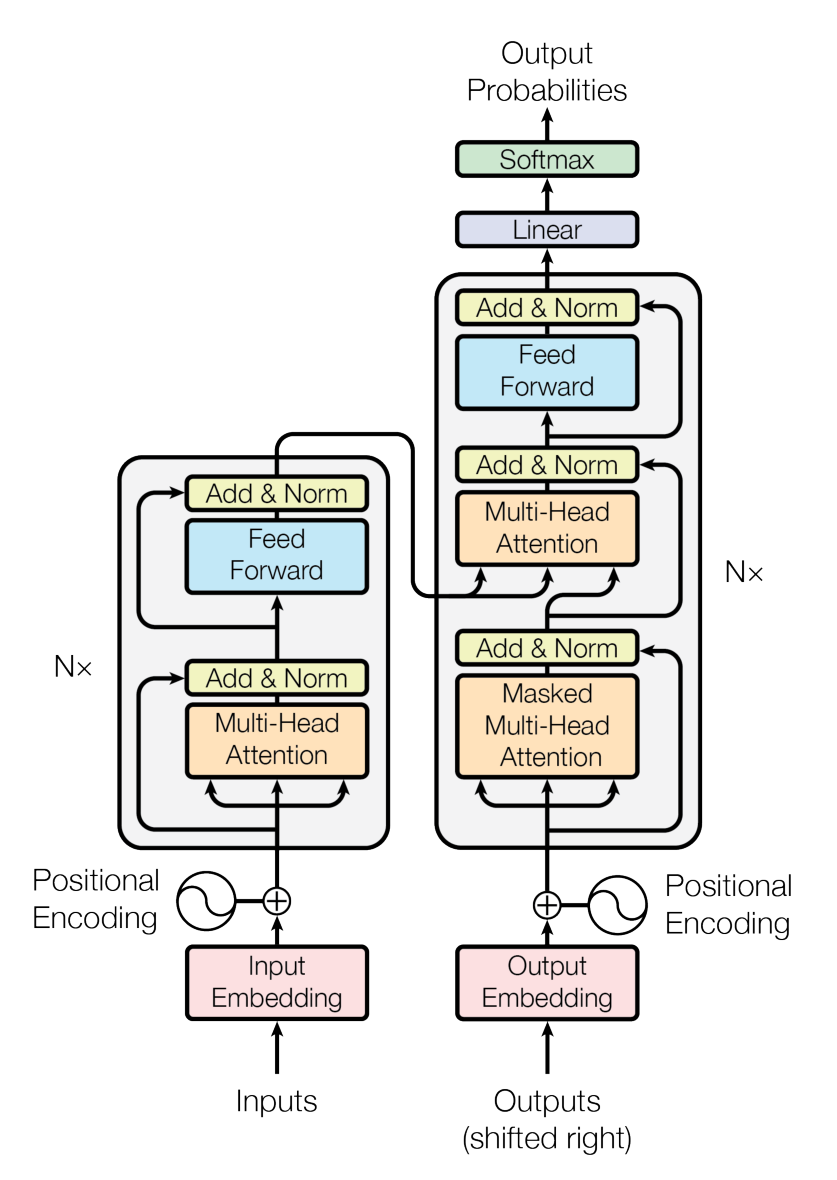
\includegraphics[width=0.23\textwidth]{transformer-architecture.png}
    \label{transformer-architecture}
  \end{figure}
  \begin{center}%
    \tiny Архитектура Transformer из статьи «Attention is all you need»
  \end{center}
\end{frame}


\begin{frame}[fragile]{Механизм внимания}%
  Механизм внимания может быть представлен формулой:
  \begin{equation}\label{scaled-dot-product-attention}%
    \operatorname{Attention}(Q, K, V) = \underbrace{
      \operatorname{softmax}\left(
        \frac{QK^T}{\sqrt{d_k}}
      \right)
    }_{\text{scores}}
    V,
  \end{equation}
  где
  \begin{itemize}%
    \item scores «оценивают» важность элементов (там лежат значения от 0 до 1);
    \item $Q$ (Query), $K$ (Key), $V$ (Value) "--- матрицы входных элементов;
    \item $d_k$ "--- нижняя размерность одной из этих матриц (длина части embedding'а).
  \end{itemize}
\end{frame}


\begin{frame}[fragile]{Positional encoding}%
  Так как в Transformer'е нет ни рекурренции (recurrence), ни свёртки, нам нужно что-то, что будет использовать порядок элементов в последовательности (positional encoding):
  \begin{equation}\label{positional-encoding}%
    PE(p, 2i) = \sin\left( \frac{p}{10\,000^{2i / d_{\text{model}}}} \right),
  \end{equation}
  \begin{equation}\label{positional-encoding-2}%
    PE(p, 2i + 1) = \cos\left( \frac{p}{10\,000^{(2i + 1) / d_{\text{model}}}} \right),
  \end{equation}
  где
  \begin{itemize}%
    \item $p$ (position) "--- позиция,
    \item $i$ (dimension) "--- размер предложения.
  \end{itemize}
\end{frame}
